%
% teil1.tex -- Beispiel-File für das Paper
%
% (c) 2020 Prof Dr Andreas Müller, Hochschule Rapperswil
%
% !TEX root = ../../buch.tex
% !TEX encoding = UTF-8
%
\section{Oberflächenwellen im seichten Gewässer
\label{luke:section:SeichtenGewaesser}}
\kopfrechts{Oberflächenwellen im seichten Gewässe}

In diesem Abschnitt werden wir den Fall betrachten, dass wir eine Oberflächenwelle im seichten Gewässer haben. 
Jedoch variiert die Definition von seichten Gewässer je nach Kontext. 
Im allgemeinen nennt man Gewässer seicht, wenn diese eine große horizontale Ausdehnung in Relation zur tiefe haben. 
Dabei gibt es keine maximale Tiefe bis dort ein Gewässer als seicht angenommen wird.
In der Hydrodynamik wird von seichtem bzw. flachem Wasser gesprochen, wenn die Wellenlänge der betrachteten Wasserwelle relativ groß im Vergleich zur Tiefe ist.
Im folgendem wird ein Ansatz hergeleitet welcher aus Vereinfachungen und bekannter Formeln für seichten Gewässer besteht.
Mit dem Ansatz wird eine unbeschränkte Lösung berechnet, welche die Saint-Venant-Gleichungen ergeben.
Durch Vereinfachung der Saint-Venant-Gleichungen wird die nichtlineare partielle Differenzialgleichung von Burger hergeleitet, sowie Rückschlüsse auf die Lösung der allgemeinen nichtlinearen eindimensionalen Wellengleichung werden gezogen. 

\subsection{Wahl eines einfachen Ansatzes}
Zuerst definieren wir das Geschwindigkeitsfeld $\bm{u}(\bm{x},z,t)$ bzw. die Ausbreitung der Welle entlang der Horizontale.
Dabei stößt man in der Literatur auf folgende Reihenentwicklung welche sich dafür bewährt hat:
\[
\bm{u}(\bm{x},z,t) = \check{\bm{u}}(\bm{x},z,t) - \frac{1}{2} (z + h)^2 \nabla^2 \check{\bm{u}}(\bm{x},z,t) + \frac{1}{24} (z + h)^4 \nabla^4 \check{\bm{u}}(\bm{x},z,t) + \ldots
\]
Die Entwicklung beschreibt eine lange Welle in seichten Wasser welche sich entlang eines horizontalen undurchlässigen Boden bei $z = -h$ ausbreitet.

Um die Berechnungen einfach zu halten wird für die Funktionen $\phi (\bm{x},z,t)$ und $\bm{u} (\bm{x},z,t)$, in Bezug auf die vertikale Richtung $z$, als konstant angenähert, durch die mittelung über die Wassertiefe \eqref{luke:Mittelung_Wassertiefe}.
Die Funktion $v$ wird auch als lineare in Bezug auf $z$ angenähert. 
Konkret erhalten wir dadurch folgenden Ansatz für die Geschwindigkeit:
\begin{equation}
	\phi(\bm{x},z,t) \approx \bar{\phi}(\bm{x}, t), \quad \bm{u}(\bm{x},z,t) \approx \bar{\bm{u}}(\bm{x}, t), \quad v(\bm{x},z,t) \approx \left(\frac{z + h}{\eta + h}\right) \tilde{v}(\bm{x}, t).
	\label{luke:Ansatz_Geschw}
\end{equation}
Dieser Ansatz findet oft in der Modellierung von seichten Gewässern Verwendung, weil dieser gut die Bewegung des Wassers in der Nähe der Oberfläche beschreibt.
Die Lagrange-Multiplikatoren $\mu(\bm{x},z,t)$ und $\nu(\bm{x},z,t)$ werden ebenfalls entsprechend diesem Ansatz angenähert:
\begin{equation}
	\quad \bm{\mu}(\bm{x},z,t) \approx \bar{\bm{\mu}}(\bm{x}, t), \quad \upsilon(\bm{x},z,t) \approx \left(\frac{z + h}{\eta(\bm{x}, t) + h}\right)\tilde{\upsilon}(\bm{x}, t).
	\label{luke:Ansatz_Multiplikatoren}
\end{equation}
Die beiden Ansätze \eqref{luke:Ansatz_Geschw} und \eqref{luke:Ansatz_Multiplikatoren} werden in die Lagrange-Funktion \eqref{luke:Luke_Lagrangian_umgeschrieben} eingefügt.
Damit wird die Lagrange-Funktion zu:
\[
L(x,y,z,t,\eta,\phi,\bm{u}, v, \bm{\mu},\upsilon,\phi_t,\phi_x,\phi_y,\phi_z)
=
\]
\[
\left(\frac{\partial \eta(\bm{x}, t)}{\partial t}
+
\bar{\bm{\mu}}  \nabla \eta(\bm{x}, t)
-
\widetilde{\upsilon}\right) \bar{\phi}
-
\frac{1}{2} g \eta(\bm{x}, t)^2
\]
\[
+
\int_{-h}^{\eta(\bm{x}, t)} \Bigg[ \bar{\bm{\mu}}  \bar{\bm{u}} - \frac{1}{2} \bar{\bm{u}}^2 +\left(\frac{z + h}{\eta(\bm{x}, t) + h}\right)\tilde{\upsilon} \left(\frac{z + h}{\eta(\bm{x}, t) + h}\right)\tilde{v} - \frac{1}{2} \left(\frac{z + h}{\eta(\bm{x}, t) + h}\right)\tilde{v}^2 
\]
\[
+\left(\nabla \bar{\bm{\mu}} + \frac{\partial}{\partial z} \left(\frac{z + h}{\eta(\bm{x}, t) + h}\right)\tilde{\upsilon}\right) \bar{\phi} \Bigg] dz.
\]

Das Integral wird umgeformt und für das vereinfachte Verständnis auf drei Teile aufgeteilt:
\[
=
\left(\frac{\partial \eta(\bm{x}, t)}{\partial t}
+
\bar{\bm{\mu}}  \nabla \eta(\bm{x}, t)
-
\widetilde{\upsilon}\right) \bar{\phi}
-
\frac{1}{2} g \eta(\bm{x}, t)^2
\]
\[
+
\int_{-h}^{\eta(\bm{x}, t)} \left[ \nabla \bar{\bm{\mu}}\bar{\phi} + \bar{\bm{\mu}}\bar{\bm{u}} - \frac{1}{2} \bar{\bm{u}}^2\right] dz
+
\int_{-h}^{\eta(\bm{x}, t)} \left[ \left(\frac{z + h}{\eta(\bm{x}, t) + h}\right)^2 \left(\tilde{\upsilon}\tilde{v} - \frac{1}{2} \tilde{v}^2\right)\right] dz
\]
\[
+
\int_{-h}^{\eta(\bm{x}, t)} \left[ \left(\frac{\partial}{\partial z} \left(\frac{z + h}{\eta(\bm{x}, t) + h}\right)\tilde{\upsilon} \bar{\phi} \right)\right] dz.
\]
Die drei Integrale werden aufgelöst wobei $\left(\frac{\partial}{\partial z} \left(\frac{z + h}{\eta(\bm{x}, t) + h}\right)\tilde{\upsilon} \bar{\phi} \right) = \frac{\tilde{\upsilon} \bar{\phi}}{\eta(\bm{x}, t) + h}$ ist:
\[
=
\left(\frac{\partial \eta(\bm{x}, t)}{\partial t}
+
\bar{\bm{\mu}} \nabla \eta(\bm{x}, t)
-
\widetilde{\upsilon}\right) \bar{\phi}
-
\frac{1}{2} g \eta(\bm{x}, t)^2
+
(\eta(\bm{x}, t) + h) \left(\nabla \bar{\bm{\mu}}\bar{\phi} + \bar{\bm{\mu}}\bar{\bm{u}} - \frac{1}{2} \bar{\bm{u}}^2\right)
\]
\[
+
(\eta(\bm{x}, t) + h) \left(\frac{1}{3}\tilde{\upsilon}\tilde{v} - \frac{1}{6}\tilde{v}^2 \right)
+
\tilde{\upsilon} \bar{\phi}.
\]
Somit erhalten wir folgende einfache Lagrangian-Funktion für eine Oberflächenwasserwelle in seichten Gewässer:
\[
L(x,y,z,t,\eta,\phi,\bm{u}, v, \bm{\mu},\upsilon,\phi_t,\phi_x,\phi_y,\phi_z)
=
\]
\[
\left(\frac{\partial \eta(\bm{x}, t)}{\partial t}
+
\bar{\bm{\mu}} \nabla \eta(\bm{x}, t) \right) \bar{\phi}
-
\frac{1}{2} g \eta(\bm{x}, t)^2
\]
\begin{equation}
	+
	(\eta(\bm{x}, t) + h) \left(\nabla \bar{\bm{\mu}}\bar{\phi} + \bar{\bm{\mu}}\bar{\bm{u}} - \frac{1}{2} \bar{\bm{u}}^2 + \frac{1}{3} \tilde{\upsilon}\tilde{v} - \frac{1}{6}\tilde{v}^2\right)
	\label{luke:Lagrangian_mit_Ansatz}
\end{equation}

Im nächsten Schritt werden wir diesen Lagrangian \eqref{luke:Lagrangian_mit_Ansatz} nehmen und das Variationsprinzip anwenden.

\subsection{Berechnung der unbeschränkte Lösung}

Ohne weitere Einschränkungen werden wir nun die Minimierung über das Variationsprinzip durchführen und folgende Euler-Lagrange-Gleichungen aufstellen:

\[
\frac{\partial \mathscr{L}}{\partial \bar{\bm{u}}} = 0
,\quad
\frac{\partial \mathscr{L}}{\partial \bar{\bm{\mu}}} = 0
,\quad
\frac{\partial \mathscr{L}}{\partial \tilde{v}} = 0
,\quad
\frac{\partial \mathscr{L}}{\partial \tilde{\upsilon}} = 0
,\quad
\frac{\partial \mathscr{L}}{\partial \bar{\phi}} = 0
,\quad
\frac{\partial \mathscr{L}}{\partial \eta} = 0
\]
%Variation nach u
\[
\frac{\partial \mathscr{L}}{\partial \bar{\bm{u}}}
=
\frac{\partial \mathscr{}}{\partial \bar{\bm{u}}}\left((\eta + h) (\bar{\bm{\mu}}\bar{\bm{u}} - \frac{1}{2} \bar{\bm{u}}^2)\right)
= 0
\]

\begin{equation}
	\frac{\partial \mathscr{L}}{\partial \bar{\bm{u}}}
	=
	\bar{\bm{\mu}} - \bar{\bm{u}}
	= 0
	\label{luke:Variation_nach_u}
\end{equation}

%Variation nach mu
\[
\frac{\partial \mathscr{L}}{\partial \bar{\bm{\mu}}}
=
\frac{\partial \mathscr{}}{\partial \bar{\bm{\mu}}} \left( \bar{\bm{\mu}} \nabla \eta \bar{\phi}+(\eta + h) (\nabla \bar{\bm{\mu}}\bar{\phi}+\bar{\bm{\mu}}\bar{\bm{u}}) \right)
= 0
\]

\begin{equation}
	\frac{\partial \mathscr{L}}{\partial \bar{\bm{\mu}}}
	=
	???
	= 0
	\label{luke:Variation_nach_mu}
\end{equation}

%Variation nach v
\[
\frac{\partial \mathscr{L}}{\partial \tilde{v}}
=
\frac{\partial \mathscr{}}{\partial \tilde{v}}\left((\eta + h) (\frac{1}{3} \tilde{\upsilon}\tilde{v} - \frac{1}{6} \tilde{v}^2)\right)
= 0
\]

\begin{equation}
	\frac{\partial \mathscr{L}}{\partial \tilde{v}}
	=
	\tilde{\upsilon}-\tilde{v}
	= 0
	\label{luke:Variation_nach_v}
\end{equation}

%Variation nach upsilon
\[
\frac{\partial \mathscr{L}}{\partial \tilde{\upsilon}}
=
\frac{\partial \mathscr{}}{\partial \tilde{\upsilon}}\left((\eta + h) (\frac{1}{3} \tilde{\upsilon}\tilde{v})\right)
= 0
\]

\begin{equation}
	\frac{\partial \mathscr{L}}{\partial \tilde{\upsilon}}
	=
	\tilde{v}
	= 0
	\label{luke:Variation_nach_upsilon}
\end{equation}

%Variation nach phi
\[
\frac{\partial \mathscr{L}}{\partial \bar{\phi}}
=
\frac{\partial \mathscr{}}{\partial \bar{\phi}}\left( (\frac{\partial \eta}{\partial t} + \bar{\bm{\mu}} \nabla \eta) \bar{\phi} + (\eta + h) \nabla \bar{\bm{\mu}}\bar{\phi}\right)
= 0
\]
\begin{equation}
	\frac{\partial \mathscr{L}}{\partial \bar{\phi}}
	=
	\frac{\partial \eta}{\partial t} + \bar{\bm{\mu}} \nabla \eta + (\eta + h) \nabla \bar{\bm{\mu}}
	= 0
	\label{luke:Variation_nach_phi}
\end{equation}

%Variation nach eta
\[
\frac{\partial \mathscr{L}}{\partial \eta}
=
\frac{\partial \mathscr{}}{\partial \eta}
\left(
\frac{\partial \eta}{\partial t} \bar{\phi}
+
\bar{\bm{\mu}}\nabla\eta\bar{\phi}
-
\frac{1}{2} g \eta^2
+
\eta \left(\nabla \bar{\bm{\mu}}\bar{\phi} + \bar{\bm{\mu}}\bar{\bm{u}} - \frac{1}{2} \bar{\bm{u}}^2 + \frac{1}{3} \tilde{\upsilon}\tilde{v} - \frac{1}{6}\tilde{v}^2\right)
\right)
= 0
\]
\begin{equation}
	\frac{\partial \mathscr{L}}{\partial \eta}
	=
	???
	= 0.
	\label{luke:Variation_nach_eta}
\end{equation}

Wie zu erwarten ergibt die Gleichung \eqref{luke:Variation_nach_u} und \eqref{luke:Variation_nach_v} das $\bar{\bm{\mu}} = \bar{\bm{u}}$ und $\tilde{\upsilon} = \tilde{v}$ ist.
Dieser Zusammenhang wurde bereits schon beim Variieren der Lagrangian-Funktion \eqref{luke:Luke_Lagrangian_mit_Multi} gezeigt.
Die Gleichung \eqref{luke:Variation_nach_mu} und \eqref{luke:Variation_nach_upsilon} zeigen, dass die Geschwindigkeitsfelder genau einem Geschwindigkeitspotential entsprechen und das die vertikale Geschwindigkeit konstant bleibt. 
Für uns interessant sind die Gleichungen \eqref{luke:Variation_nach_phi} und \eqref{luke:Variation_nach_eta}.
Diese lassen sich nämlich umschreiben zu: 
\begin{equation}
	\frac{\partial H}{\partial t} + \nabla \cdot [H \bar{\bm{u}}] = 0
	\label{luke:Variation_loesung_1}
\end{equation}
\begin{equation}
	\frac{\partial \bar{\bm{u}}}{\partial t} + (\bar{\bm{u}} \cdot \nabla) \bar{\bm{u}} + g \nabla H = 0,
	\label{luke:Variation_loesung_2}
\end{equation}
wobei $H = \eta + h$ die Gesamtwassertiefe ist.

Gleichung \eqref{luke:Variation_loesung_1} und \eqref{luke:Variation_loesung_2} ergeben die Saint-Venant-Gleichungen.
Diese finden Verwendung bei der Modellierung von langen Wellen in unbeschränkten seichten Gewässern.
Meistens für das beschreiben von Wasserströmungen in offenen Kanälen und Flüssen.
Bei diesen Gleichungen handelt es sich um nichtlineare Differenzialgleichungen welche über verschiedene nummerischen Methoden berechnet werden können.
Da es in dieser Arbeit nicht um das numerische lösen von Differenzialgleichungen handelt, sondern um die Demonstrierung der Anwendung und Vorteile des Variationsprinzip, wird im nächsten Kapitel die Gleichung \eqref{luke:Variation_loesung_2} genauer betrachtet.
Durch Vereinfachung ergibt nämlich diese die nicht viskose Burglers-Gleichung sowie Ähnlichkeiten zur Lösung der nichtlinearen Wellengleichung im eindimensionalen Fall.

\subsection{Interpretation und Anwendung der unbeschränkten Lösung}
Wenn für die Gleichung \eqref{luke:Variation_loesung_2} angenommen wird das sich über die gesamte Zeit $t$ keine Änderung der Gesamtwassertiefe $ \nabla H = 0 $ sowie die horizontale Koordinate $y$ konstant ist $\frac{\partial \bar{\bm{u}}}{\partial y} = 0$, ergibt sich daraus die Burgers-Gleichung für ein nicht-viskoses Fluid:
\begin{equation}
	\frac{\partial \bar{u}}{\partial t} + \bar{u} \frac{\partial \bar{u}}{\partial x} = 0.
	\label{luke:Burgers_DG}
\end{equation}
Bei der Burgers-Gleichung handelt es sich um eine nichtlineare, homogene und partielle Differentialgleichung.
Die Differenzialgleichung wird in der Regel über die Charakteristikenmethode gelöst. 
Dabei entsteht folgende Lösung:
\[
\bar{u}(x,t) = f(\xi) = f(x-\bar{u}t),\quad \xi = x-f(\xi)t.
\]
wobei $\xi$ der Punkt auf der x-Achse ist bei $t = 0$ von dort aus die charakteristischen Kurve aus startet.
Diese Lösung beschreibt eine nichtlineare Wellenbewegung in welcher sich die Anfangsform der Welle im Laufe der Zeit ändert.
Sozusagen stellt dies eine Stoßwelle in x-Richtung dar.
Damit lässt sich Verhaltensweisen wie Stoßwellenbildung, Singularitäten und Schockwellen beschreiben.
\begin{figure}
	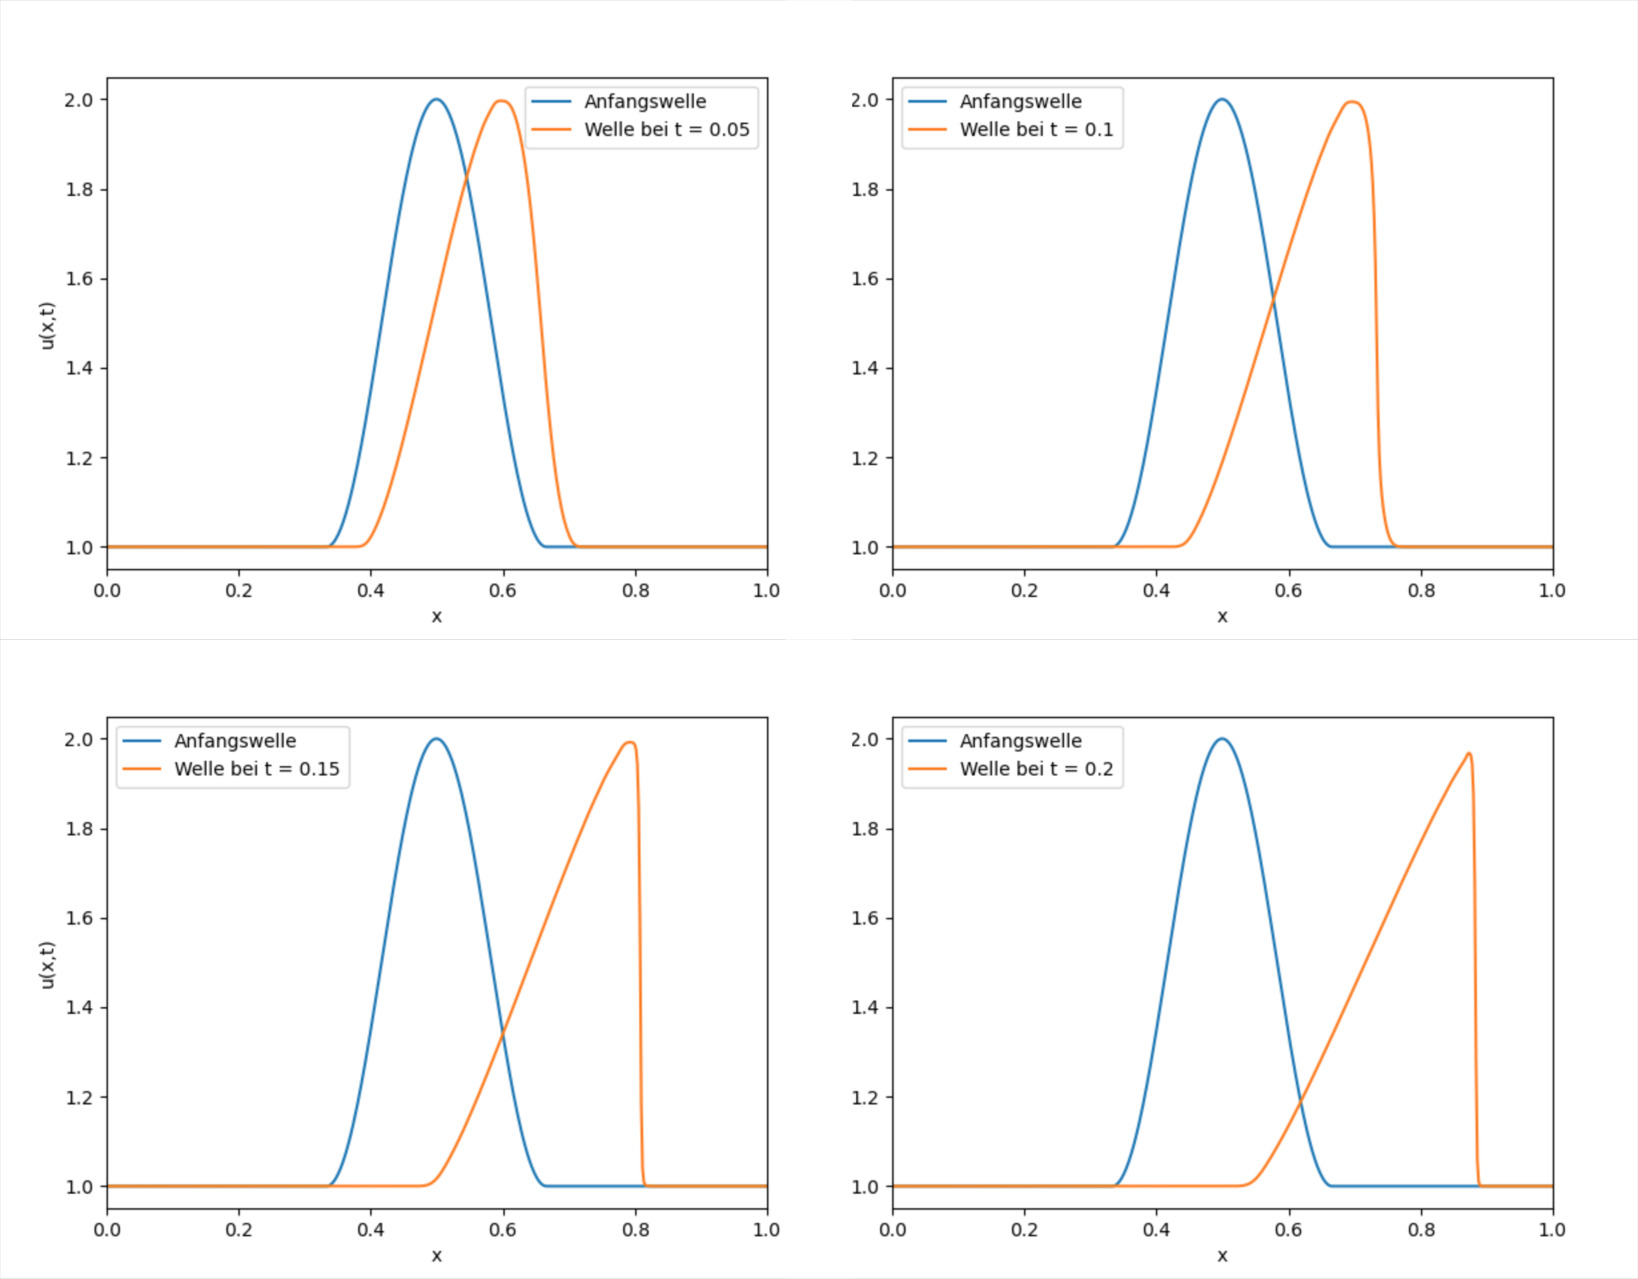
\includegraphics[width=\textwidth]{papers/luke/fig/Burger_Loesung_Welle.jpg}
	\caption{Lösung der Burgers Differenzialgleichung \eqref{luke:Burgers_DG} mit einem $sin(x)^2$ als Welle
		\label{luke:fig:Loesung_Burgers}}
\end{figure}
Graphik \ref{luke:fig:Loesung_Burgers} zeigt die Lösung der Burger-Gleichung mit einer fortlaufenden Welle welche zu einem Überschlag der Welle führt.

Die allgemeine nichtlineare Wellengleichung in einer Dimension lautet:
\[
\partial_t^2 u - a^2 \partial_x^2 u  = 0.
\]
Dabei ist $a$ die Geschwindigkeit der Welle entlang der x-Achse.
Diese Wellengleichung kann in einem Bereich von $\Omega = \{(x,t)\mid t >0\}$ gelöst werden mit folgenden Anfangswerte:
\[
u(x,0) = u_0(x),\quad \frac{\partial u}{\partial t} = v_0(x),\quad x \in \mathbb{R}.
\]
Wenn angenommen wird das die Geschwindigkeit $a$ konstant ist, kann die Gleichung auf folgende Differenzialgleichung erster Ordnung umgeschrieben werden:
\[
(\partial_t\mp a\partial_x)(\partial_t\pm a\partial_x) u  = 0.
\]
Somit ist die Lösung dieser Gleichung erster Ordnung:
\begin{equation}
	\partial_t u \mp a\partial_x u = 0
	\label{luke:Loesung_Wellengleichung}
\end{equation}
automatisch eine Lösung der Wellengleichung.
Wenn nun die Gleichung \eqref{luke:Variation_loesung_2} hergenommen wird, welche über das Variationsprinzip berechnet wurde, und erneut angenommen wird das sich über die gesamte Zeit $t$ keine Änderung der Gesamtwassertiefe $ \nabla H = 0 $ sowie die horizontale Koordinate $y$ konstant ist, und diese mit der Lösung der Wellengleichung \eqref{luke:Loesung_Wellengleichung} verglichen wird,
\[
\text{Variation: }\frac{\partial \bar{u}}{\partial t} + \bar{u} \frac{\partial \bar{u}}{\partial x} = 0,
\qquad
\text{Wellengleichung: }\frac{\partial u}{\partial t} + a \frac{\partial u}{\partial x} = 0,
\]
dann ist zu erkennen, dass sich die Lösung über die Variation von der Lösung der Wellengleichung anhand wie die Geschwindigkeit der Welle eingebunden ist unterscheidet.
Bei der Wellengleichung ist die Wellengeschwindigkeit $a$ eine Konstante, wobei es bei der Lösung der Variation die Wellengeschwindigkeit $\bar{u}$ von der Position $x$ sowie der Zeit $t$ abhängig ist.
